\documentclass[a4paper]{report}
\usepackage{longtable,float,hyperref,color,amsmath,amsxtra,amssymb,latexsym,amscd,amsthm,amsfonts,graphicx,enumitem,parskip,imakeidx}
\usepackage{tikz,graphicx}
\usetikzlibrary{shapes,arrows}
\usetikzlibrary{calc}
\usetikzlibrary{decorations.pathreplacing,angles,quotes}
%\numberwithin{equation}{section}
%\allowdisplaybreaks
%\usepackage{fancyhdr}
%\pagestyle{fancy}
%\fancyhf{}
%\fancyhead[RE,LO]{\footnotesize \textsc \leftmark}
%\cfoot{\thepage}
%\renewcommand{\headrulewidth}{0.5pt}
%\setcounter{tocdepth}{1}
%\setcounter{secnumdepth}{1}
\usepackage[utf8x]{inputenc}
%\setlength\parindent{0pt}
\makeindex[columns=2, title=Alphabetical Index, 
           options= -s index.ist]
\title{\Huge Homework Assignment\\Differential Geometry}
\author{\textsc{Nguyen Quan Ba Hong}\\
	{\small \texttt{MSSV: 1411103}}\\
	\textsc{Nguyen An Thinh}\\
	{\small \texttt{MSSV: 1411289}}\\
	\textsc{Doan Tran Nguyen Tung}\\
{\small \texttt{MSSV: 1411352}}}

\begin{document}
\maketitle
\textbf{Problem:} If a circle if rolled along a line (without friction), then a fixed point on that circle has its trajectory as the so-called \textit{cycloid}.
\begin{enumerate}[label=(\alph*), leftmargin=*]
	\item\label{a} Find a parameterization for the cycloid.
	\item\label{b} Compute the curvature of the cycloid.
\end{enumerate}

\textsc{Solution}

To find a parameterization for the cycloid, we should have some intuition about it through the following figure.
\begin{figure}[H]
	\centering
	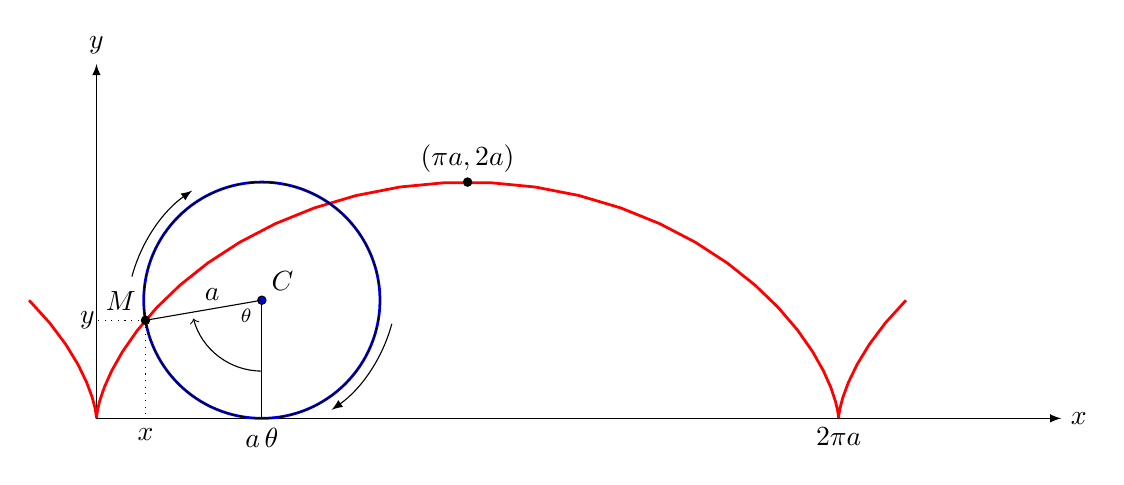
\begin{tikzpicture}[scale=1.5]
	\coordinate (O) at (0,0);
	\coordinate (A) at (0,3);
	\def\r{1} % radius
	\def\c{1.4} % center
	\coordinate (C) at (\c, \r);
	
	
	\draw[-latex] (O) -- (A) node[anchor=south] {$y$};
	\draw[-latex] (O) -- (2.6*pi,0) node[anchor=west] {$x$};
	\draw[red,domain=-0.5*pi:2.5*pi,samples=50, line width=1] 
	plot ({\x - sin(\x r)},{1 - cos(\x r)});
	\draw[blue, line width=1] (C) circle (\r);
	\draw[] (C) circle (\r);
	
	% coordinate x 
	\def\x{0.415} % coordinate x
	\def\y{0.83} % coordinate y
	\def\xa{0.3} % coordinate x for arc left
	\def\ya{1.2} % coordinate y for arc left
	\coordinate (X) at (\x, 0 );
	\coordinate (Y) at (0, \y );
	\coordinate (XY) at (\x, \y );
	
	\node[anchor=north] at (X) {$x$} ;
	
	% draw center of circle
	\draw[fill=blue] (C) circle (1pt);
	
	% draw radius of the circle
	\draw[] (C) -- node[anchor=south] {\; $a$} (XY);
	\node[anchor=south west] at (C) {$C$};
	
	% bottom of circle, radius to the bottom
	\coordinate (B) at (\c, 0);
	\draw[] (C) -- (B) node[anchor=north] {$a \, \theta$};
	
	% projections of point XY
	\draw[dotted] (XY) -- (X);
	\draw[dotted] (XY) -- (Y) node[anchor=east, xshift=1mm] {$\quad y$};
	
	% arc theta
	% start arc
	\coordinate (S) at (\c, 0.4);
	\draw[->] (S) arc (-90:-165:0.6);
	\node[xshift=-2mm, yshift=-2mm] at (C) {\scriptsize $\theta$};
	
	% arc above
	\coordinate (AA) at (\xa, \ya);
	\draw[-latex, rotate=25] (AA) arc (-220:-260:1.3);
	
	% arc below
	\def\xb{2.5} % coordinate x for arc bottom
	\def\yb{0.8} % coordinate y for arc bottom
	\coordinate (AB) at (\xb, \yb);
	\draw[-latex, rotate=-10] (AB) arc (-5:-45:1.3);
	
	
	
	% XY dot
	\draw[fill=black] (XY) circle (1pt);
	\node[anchor=south east] at (XY) {$M$};
	
	% top label
	\coordinate (T) at (pi, 2);
	\node[anchor=south] at (T)  {$(\pi a, 2 a )$} ;
	\draw[fill=black] (T) circle (1pt);
	
%	% equations
%	\coordinate (E) at ( 4,1.2);
%	\coordinate (F) at ( 4,0.9);
%	\node[] at (E) {\scriptsize $x=a(\theta - \sin \theta)$};
%	\node[] at (F) {\scriptsize $y=a(1 - \cos \theta)$};
	
	% label 2pi a
	\coordinate (TPA) at (2*pi, 0);
	\node[anchor=north] at (TPA) {$2 \pi a$};
	\end{tikzpicture}
	\caption{A cycloid, \cite{1}}
\end{figure}
We need to find the coordinate of the point $M$ with respect to $\theta$.

First, we can see that the longitude of the center of the circle (point $C$) is the radius of the circle and the latitude is the arc length subtended by the angle $\theta$ on the circle.

Therefore, the coordinate of $C$ is $(a\theta , a)$.

As for $M$, we can denote it's coordinate as
\begin{align}
	r(\theta) = (x(\theta), y(\theta))
\end{align}
Let's consider the following cases.

\newpage
\textbf{Case 1:} $0 < \theta < \frac{\pi}{2}$
\begin{figure}[H]
	\centering
	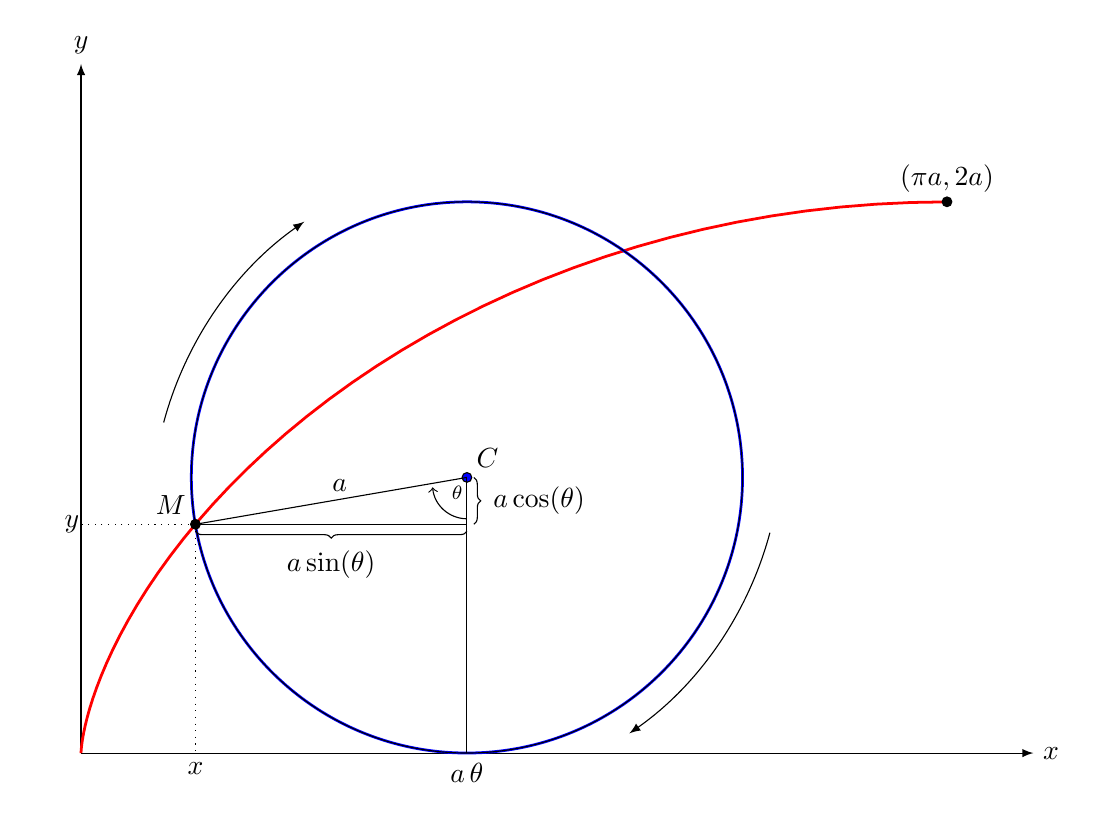
\begin{tikzpicture}[scale=3.5]
	\coordinate (O) at (0,0);
	\coordinate (A) at (0,2.5);
	\def\r{1} % radius
	\def\c{1.4} % center
	\coordinate (C) at (\c, \r);
	
	
	\draw[-latex] (O) -- (A) node[anchor=south] {$y$};
	\draw[-latex] (O) -- (1.1*pi,0) node[anchor=west] {$x$};
	\draw[red,domain=0:1*pi,samples=50, line width=1] 
	plot ({\x - sin(\x r)},{1 - cos(\x r)});
	\draw[blue, line width=1] (C) circle (\r);
	\draw[] (C) circle (\r);
	
	% coordinate x 
	\def\x{0.415} % coordinate x
	\def\y{0.83} % coordinate y
	\def\xa{0.3} % coordinate x for arc left
	\def\ya{1.2} % coordinate y for arc left
	\coordinate (X) at (\x, 0 );
	\coordinate (Y) at (0, \y );
	\coordinate (XY) at (\x, \y );
	\coordinate (XY) at (\x, \y );
	\coordinate (CY) at (\c, \y);
	
	\node[anchor=north] at (X) {$x$} ;
	
	% draw center of circle
	\draw[fill=blue] (C) circle (0.5pt);
	
	% draw radius of the circle
	\draw[] (C) -- node[anchor=south] {\; $a$} (XY);
	\node[anchor=south west] at (C) {$C$};
	
	% bottom of circle, radius to the bottom
	\coordinate (B) at (\c, 0);
	\draw[] (C) -- (B) node[anchor=north] {$a \, \theta$};
	
	% projections of point XY
	\draw[dotted] (XY) -- (X);
	\draw[dotted] (XY) -- (Y) node[anchor=east, xshift=1mm] {$\quad y$};
	
%	% arc theta
%	% start arc
	\coordinate (S) at (\c, 0.85);
	\draw[->] (S) arc (-90:-175:0.125);
	\node[xshift=-1.25mm, yshift=-2mm] at (C) {\scriptsize $\theta$};
	
	\draw[] (XY) -- (CY);
	\draw[] (C) -- (CY);
	
	\draw[decoration={brace,mirror,raise=2.5pt},decorate]
	(XY) -- node[below=6pt] {$a \sin(\theta)$} (CY);
	\draw[decoration={brace,mirror,raise=2.5pt},decorate]
	(CY) -- node[right=6pt] {$a \cos(\theta)$} (C);
	
	% arc above
	\coordinate (AA) at (\xa, \ya);
	\draw[-latex, rotate=25] (AA) arc (-220:-260:1.3);
	
	% arc below
	\def\xb{2.5} % coordinate x for arc bottom
	\def\yb{0.8} % coordinate y for arc bottom
	\coordinate (AB) at (\xb, \yb);
	\draw[-latex, rotate=-10] (AB) arc (-5:-45:1.3);
	
	
	
	% XY dot
	\draw[fill=black] (XY) circle (0.5pt);
	\node[anchor=south east] at (XY) {$M$};
	
	% top label
	\coordinate (T) at (pi, 2);
	\node[anchor=south] at (T)  {$(\pi a, 2 a )$} ;
	\draw[fill=black] (T) circle (0.5pt);
	
%	% equations
%	\coordinate (E) at ( 4,1.2);
%	\coordinate (F) at ( 4,0.9);
%	\node[] at (E) {\scriptsize $x=a(\theta - \sin \theta)$};
%	\node[] at (F) {\scriptsize $y=a(1 - \cos \theta)$};
	
%	% label 2pi a
%	\coordinate (TPA) at (2*pi, 0);
%	\node[anchor=north] at (TPA) {$2 \pi a$};
	\end{tikzpicture}
	\caption{Case 1: $0 < \theta < \frac{\pi}{2}$}
\end{figure}

%\begin{figure}[H]
%	\centering
%	\begin{tikzpicture}[scale=3.5]
%	\coordinate (O) at (0,0);
%	\coordinate (A) at (0,2.5);
%	\def\r{1} % radius
%	\def\c{1.4} % center
%	\coordinate (C) at (\c, \r);
%
%	\draw[blue, line width=1] (C) circle (\r);
%	\draw[] (C) circle (\r);
%	
%	% coordinate x 
%	\def\x{0.415} % coordinate x
%	\def\y{0.83} % coordinate y
%	\def\xa{0.3} % coordinate x for arc left
%	\def\ya{1.2} % coordinate y for arc left
%	\coordinate (X) at (\x, 0 );
%	\coordinate (Y) at (0, \y );
%	\coordinate (XY) at (\x, \y );
%	\coordinate (XY) at (\x, \y );
%	\coordinate (CY) at (\c, \y);
%	
%	% draw center of circle
%	\draw[fill=blue] (C) circle (0.5pt);
%	
%	% draw radius of the circle
%	\draw[] (C) -- node[anchor=south] {\; $a$} (XY);
%	
%	% bottom of circle, radius to the bottom
%	\coordinate (B) at (\c, 0);
%	\draw[] (C) -- (B) node[anchor=north] {$a \, \theta$};
%	
%	%	% arc theta
%	%	% start arc
%	\coordinate (S) at (\c, 0.875);
%	\draw[->] (S) arc (-90:-175:0.1);
%	\node[xshift=-1.25mm, yshift=-2mm] at (C) {\scriptsize $\theta$};
%	
%	\draw[] (XY) -- (CY);
%	\draw[] (C) -- (CY);
%	
%	\draw[decoration={brace,mirror,raise=2.5pt},decorate]
%	(XY) -- node[below=6pt] {$a \sin(\theta)$} (CY);
%	\draw[decoration={brace,mirror,raise=2.5pt},decorate]
%	(CY) -- node[right=6pt] {$a \cos(\theta)$} (C);
%
%	% XY dot
%	\draw[fill=black] (XY) circle (0.5pt);
%	\end{tikzpicture}
%	\caption{The cycloid}
%\end{figure}
From the figure, we can find the relative position of $M$ and $C$ and thus, the coordinate of $M$.
\begin{align}
	\begin{cases}
	x(\theta) &= a\theta - a\sin(\theta)\\
	&= a\left(\theta - \sin(\theta)\right)\\
	y(\theta) &= a - a\cos(\theta)\\
	 &= a\left(1 - \cos(\theta)\right)
	\end{cases}
\end{align}


\newpage
\textbf{Case 2:} $\frac{\pi}{2} < \theta < \pi$
\begin{figure}[H]
	\centering
	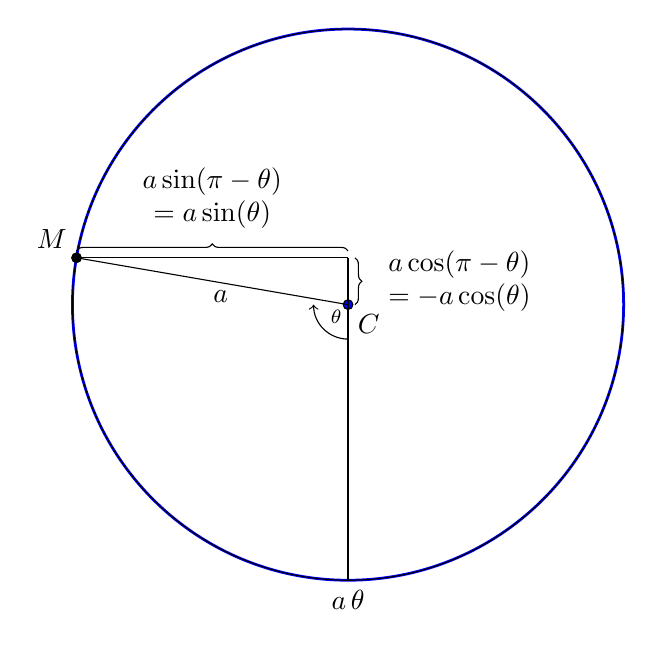
\begin{tikzpicture}[scale=3.5]
	\coordinate (O) at (0,0);
	\coordinate (A) at (0,2.5);
	\def\r{1} % radius
	\def\c{1.4} % center
	\coordinate (C) at (\c, \r);
	
	
%	\draw[-latex] (O) -- (A) node[anchor=south] {$y$};
%	\draw[-latex] (O) -- (1.1*pi,0) node[anchor=west] {$x$};
%	\draw[red,domain=0:1*pi,samples=50, line width=1] 
%	plot ({\x - sin(\x r)},{1 - cos(\x r)});
	\draw[blue, line width=1] (C) circle (\r);
	\draw[] (C) circle (\r);
	
	% coordinate x 
	\def\x{0.415} % coordinate x
	\def\y{1.17} % coordinate y
	\def\xa{0.3} % coordinate x for arc left
	\def\ya{1.2} % coordinate y for arc left
	\coordinate (X) at (\x, 0 );
	\coordinate (Y) at (0, \y );
	\coordinate (XY) at (\x, \y );
	\coordinate (XY) at (\x, \y );
	\coordinate (CY) at (\c, \y);
	
%	\node[anchor=north] at (X) {$x$} ;
	
	% draw center of circle
	\draw[fill=blue] (C) circle (0.5pt);
	
	% draw radius of the circle
	\draw[] (C) -- node[anchor=north] {\; $a$} (XY);
	\node[anchor=north west] at (C) {$C$};
	
	% bottom of circle, radius to the bottom
	\coordinate (B) at (\c, 0);
	\draw[] (C) -- (B) node[anchor=north] {$a \, \theta$};
	
	%	% arc theta
	%	% start arc
	\coordinate (S) at (\c, 0.875);
	\draw[->] (S) arc (-90:-180:0.125);
	\node[xshift=-1.5mm, yshift=-1.5mm] at (C) {\scriptsize $\theta$};
	
	\draw[] (XY) -- (CY);
	\draw[] (C) -- (CY);
	
	\draw[decoration={brace,mirror,raise=2.5pt},decorate]
	(CY) -- node[above=6pt] {$\begin{array}{c}
		a \sin(\pi - \theta)\\
		= a \sin(\theta)
		\end{array}$} (XY);
	\draw[decoration={brace,mirror,raise=2.5pt},decorate]
	(C) -- node[right=6pt] {$\begin{array}{c}
		a \cos(\pi - \theta)\\ 
		= - a \cos(\theta)
		\end{array} $} (CY);
	
	% XY dot
	\draw[fill=black] (XY) circle (0.5pt);
	\node[anchor=south east] at (XY) {$M$};
	\end{tikzpicture}
	\caption{Case 2: $\frac{\pi}{2} < \theta < \pi$}
\end{figure}
From the figure, we can find the coordinate of $M$ as
\begin{align}
\begin{cases}
x(\theta) &= a\theta - a\sin(\theta)\\
&= a\left(\theta - \sin(\theta)\right)\\
y(\theta) &= a + \left(- a\cos(\theta)\right)\\
&= a\left(1 - \cos(\theta)\right)
\end{cases}
\end{align}


\newpage
\textbf{Case 3:} $\pi < \theta < \frac{3\pi}{2}$
\begin{figure}[H]
	\centering
	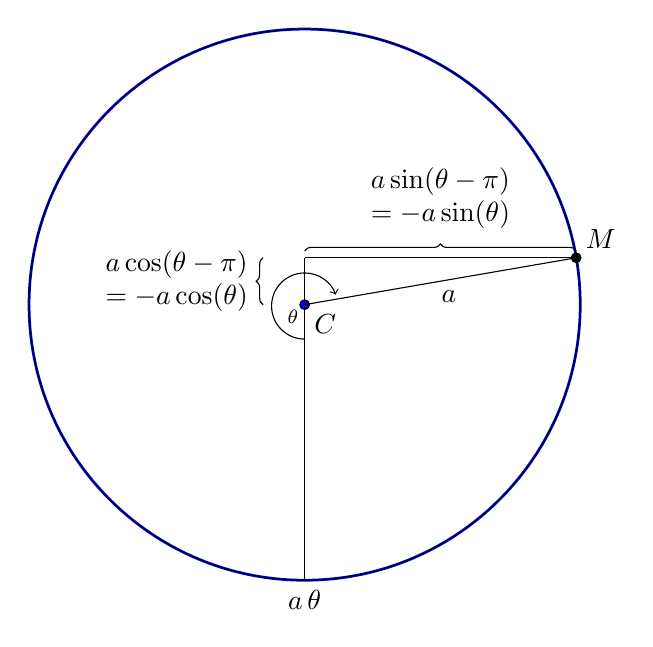
\begin{tikzpicture}[scale=3.5]
	\coordinate (O) at (0,0);
	\coordinate (A) at (0,2.5);
	\def\r{1} % radius
	\def\c{-0.57} % center
	\coordinate (C) at (\c, \r);
	
	
	%	\draw[-latex] (O) -- (A) node[anchor=south] {$y$};
	%	\draw[-latex] (O) -- (1.1*pi,0) node[anchor=west] {$x$};
	%	\draw[red,domain=0:1*pi,samples=50, line width=1] 
	%	plot ({\x - sin(\x r)},{1 - cos(\x r)});
	\draw[blue, line width=1] (C) circle (\r);
	\draw[] (C) circle (\r);
	
	% coordinate x 
	\def\x{0.415} % coordinate x
	\def\y{1.17} % coordinate y
	\def\xa{0.3} % coordinate x for arc left
	\def\ya{1.2} % coordinate y for arc left
	\coordinate (X) at (\x, 0 );
	\coordinate (Y) at (0, \y );
	\coordinate (XY) at (\x, \y );
	\coordinate (XY) at (\x, \y );
	\coordinate (CY) at (\c, \y);
	
	%	\node[anchor=north] at (X) {$x$} ;
	
	% draw center of circle
	\draw[fill=blue] (C) circle (0.5pt);
	
	% draw radius of the circle
	\draw[] (C) -- node[anchor=north] {\; $a$} (XY);
	\node[anchor=north west] at (C) {$C$};
	
	% bottom of circle, radius to the bottom
	\coordinate (B) at (\c, 0);
	\draw[] (C) -- (B) node[anchor=north] {$a \, \theta$};
	
	%	% arc theta
	%	% start arc
	\coordinate (S) at (\c, 0.875);
	\draw[->] (S) arc (-90:-340:0.12);
	\node[xshift=-1.5mm, yshift=-1.5mm] at (C) {\scriptsize $\theta$};
	
	\draw[] (XY) -- (CY);
	\draw[] (C) -- (CY);
	
	\draw[decoration={brace,mirror,raise=2.5pt},decorate]
	(XY) -- node[above=6pt] {$\begin{array}{c}
		a \sin(\theta - \pi)\\
		= - a \sin(\theta)
		\end{array}$} (CY);
	\draw[decoration={brace,mirror,raise=15pt},decorate]
	(CY) -- node[left=12pt] {$\begin{array}{c}
		a \cos(\theta - \pi)\\ 
		= - a \cos(\theta)
		\end{array} $} (C);
	
	% XY dot
	\draw[fill=black] (XY) circle (0.5pt);
	\node[anchor=south west] at (XY) {$M$};
	\end{tikzpicture}
	\caption{Case 3: $\pi < \theta < \frac{3\pi}{2}$}
\end{figure}
From the figure, we can find the coordinate of $M$ as
\begin{align}
\begin{cases}
x(\theta) &= a\theta +  \left(- a\sin(\theta)\right)\\
&= a\left(\theta - \sin(\theta)\right)\\
y(\theta) &= a\theta + \left(- a\cos(\theta)\right)\\
&= a\left(1 - \cos(\theta)\right)
\end{cases}
\end{align}

\newpage
\textbf{Case 4:} $\frac{3\pi}{2} < \theta < 2\pi$
\begin{figure}[H]
	\centering
	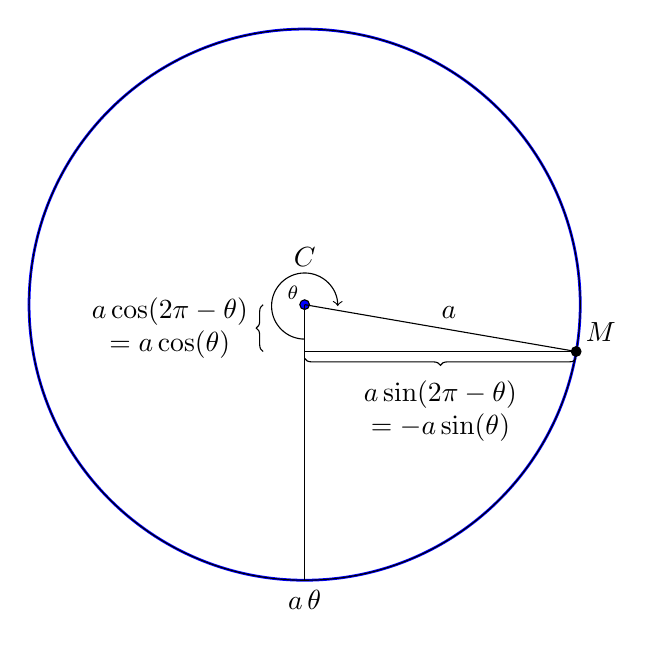
\begin{tikzpicture}[scale=3.5]
	\coordinate (O) at (0,0);
	\coordinate (A) at (0,2.5);
	\def\r{1} % radius
	\def\c{-0.57} % center
	\coordinate (C) at (\c, \r);
	
	
	%	\draw[-latex] (O) -- (A) node[anchor=south] {$y$};
	%	\draw[-latex] (O) -- (1.1*pi,0) node[anchor=west] {$x$};
	%	\draw[red,domain=0:1*pi,samples=50, line width=1] 
	%	plot ({\x - sin(\x r)},{1 - cos(\x r)});
	\draw[blue, line width=1] (C) circle (\r);
	\draw[] (C) circle (\r);
	
	% coordinate x 
	\def\x{0.415} % coordinate x
	\def\y{0.83} % coordinate y
	\def\xa{0.3} % coordinate x for arc left
	\def\ya{1.2} % coordinate y for arc left
	\coordinate (X) at (\x, 0 );
	\coordinate (Y) at (0, \y );
	\coordinate (XY) at (\x, \y );
	\coordinate (XY) at (\x, \y );
	\coordinate (CY) at (\c, \y);
	
	%	\node[anchor=north] at (X) {$x$} ;
	
	% draw center of circle
	\draw[fill=blue] (C) circle (0.5pt);
	
	% draw radius of the circle
	\draw[] (C) -- node[anchor=south] {\; $a$} (XY);
	\node[xshift=0mm, yshift=6mm] at (C) {$C$};
	
	% bottom of circle, radius to the bottom
	\coordinate (B) at (\c, 0);
	\draw[] (C) -- (B) node[anchor=north] {$a \, \theta$};
	
	%	% arc theta
	%	% start arc
	\coordinate (S) at (\c, 0.875);
	\draw[->] (S) arc (-90:-360:0.12);
	\node[xshift=-1.5mm, yshift=1.5mm] at (C) {\scriptsize $\theta$};
	
	\draw[] (XY) -- (CY);
	\draw[] (C) -- (CY);
	
	\draw[decoration={brace,mirror,raise=2.5pt},decorate]
	(CY) -- node[below=6pt] {$\begin{array}{c}
		a \sin(2\pi - \theta)\\
		= - a \sin(\theta)
		\end{array}$} (XY);
	\draw[decoration={brace,mirror,raise=15pt},decorate]
	(C) -- node[left=12pt] {$\begin{array}{c}
		a \cos(2\pi - \theta)\\ 
		= a \cos(\theta)
		\end{array} $} (CY);
	
	% XY dot
	\draw[fill=black] (XY) circle (0.5pt);
	\node[anchor=south west] at (XY) {$M$};
	\end{tikzpicture}
	\caption{Case 4: $\frac{3\pi}{2} < \theta < 2\pi$}
\end{figure}
From the figure, we can find the coordinate of $M$ as
\begin{align}
\begin{cases}
x(\theta) &= a\theta + \left( - a\sin(\theta)\right)\\
&= a\left(\theta - \sin(\theta)\right)\\
y(\theta) &= a - a\cos(\theta)\\
&= a\left(1 - \cos(\theta)\right)
\end{cases}
\end{align}

\newpage
\textbf{Case 5:} $\theta = 0\pi$
\begin{figure}[H]
	\centering
	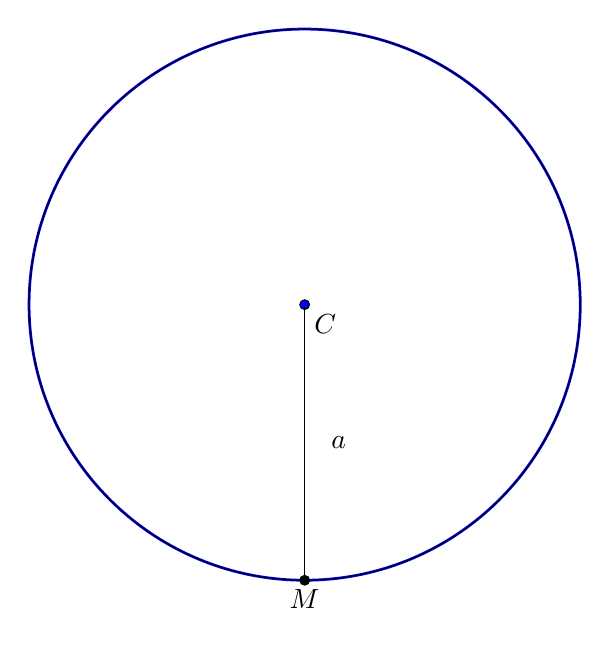
\begin{tikzpicture}[scale=3.5]
	\coordinate (O) at (0,0);
	\coordinate (A) at (0,2.5);
	\def\r{1} % radius
	\def\c{1.4} % center
	\coordinate (C) at (\c, \r);
	
	
	%	\draw[-latex] (O) -- (A) node[anchor=south] {$y$};
	%	\draw[-latex] (O) -- (1.1*pi,0) node[anchor=west] {$x$};
	%	\draw[red,domain=0:1*pi,samples=50, line width=1] 
	%	plot ({\x - sin(\x r)},{1 - cos(\x r)});
	\draw[blue, line width=1] (C) circle (\r);
	\draw[] (C) circle (\r);
	
	% coordinate x 
	\def\x{1.4} % coordinate x
	\def\y{0} % coordinate y
	\def\xa{0.3} % coordinate x for arc left
	\def\ya{1.2} % coordinate y for arc left
	\coordinate (X) at (\x, 0 );
	\coordinate (Y) at (0, \y );
	\coordinate (XY) at (\x, \y );
	\coordinate (XY) at (\x, \y );
	\coordinate (CY) at (\c, \y);
	
	%	\node[anchor=north] at (X) {$x$} ;
	
	% draw center of circle
	\draw[fill=blue] (C) circle (0.5pt);
	
	% draw radius of the circle
	\draw[] (C) -- node[anchor=west] {\; $a$} (XY);
	\node[anchor=north west] at (C) {$C$};
	
	% XY dot
	\draw[fill=black] (XY) circle (0.5pt);
	\node[anchor=north] at (XY) {$M$};
	\end{tikzpicture}
	\caption{Case 5: $\theta = 0\pi$}
\end{figure}
In this case, we can see that
\begin{align}
\begin{cases}
\sin(\theta) &= 0\\
\cos(\theta) &= 1
\end{cases}
\end{align}
Therefore, the coordinate of $M$ is
\begin{align}
\begin{cases}
x(\theta) &= 0 = a\left(\theta - \sin(\theta)\right)\\
y(\theta) &= 0 = a\left(1 - \cos(\theta)\right)
\end{cases}
\end{align}

\newpage
\textbf{Case 6:} $\theta = \frac{\pi}{2}$
\begin{figure}[H]
	\centering
	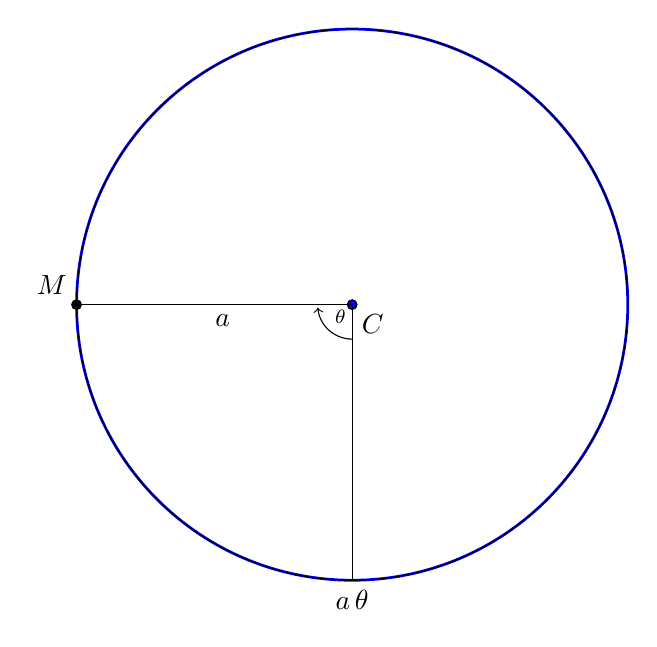
\begin{tikzpicture}[scale=3.5]
	\coordinate (O) at (0,0);
	\coordinate (A) at (0,2.5);
	\def\r{1} % radius
	\def\c{1.4} % center
	\coordinate (C) at (\c, \r);
	
	
	%	\draw[-latex] (O) -- (A) node[anchor=south] {$y$};
	%	\draw[-latex] (O) -- (1.1*pi,0) node[anchor=west] {$x$};
	%	\draw[red,domain=0:1*pi,samples=50, line width=1] 
	%	plot ({\x - sin(\x r)},{1 - cos(\x r)});
	\draw[blue, line width=1] (C) circle (\r);
	\draw[] (C) circle (\r);
	
	% coordinate x 
	\def\x{0.4} % coordinate x
	\def\y{1} % coordinate y
	\def\xa{0.3} % coordinate x for arc left
	\def\ya{1.2} % coordinate y for arc left
	\coordinate (X) at (\x, 0 );
	\coordinate (Y) at (0, \y );
	\coordinate (XY) at (\x, \y );
	\coordinate (XY) at (\x, \y );
	\coordinate (CY) at (\c, \y);
	
	%	\node[anchor=north] at (X) {$x$} ;
	
	% draw center of circle
	\draw[fill=blue] (C) circle (0.5pt);
	
	% draw radius of the circle
	\draw[] (C) -- node[anchor=north] {\; $a$} (XY);
	\node[anchor=north west] at (C) {$C$};
	
	% bottom of circle, radius to the bottom
	\coordinate (B) at (\c, 0);
	\draw[] (C) -- (B) node[anchor=north] {$a \, \theta$};
	
	%	% arc theta
	%	% start arc
	\coordinate (S) at (\c, 0.875);
	\draw[->] (S) arc (-90:-175:0.125);
	\node[xshift=-1.5mm, yshift=-1.5mm] at (C) {\scriptsize $\theta$};
	
	% XY dot
	\draw[fill=black] (XY) circle (0.5pt);
	\node[anchor=south east] at (XY) {$M$};
	\end{tikzpicture}
	\caption{Case 6: $\theta = \frac{\pi}{2}$}
\end{figure}
In this case, we can see that
\begin{align}
\begin{cases}
\sin(\theta) &= 1\\
\cos(\theta) &= 0
\end{cases}
\end{align}
Therefore, the coordinate of $M$ is
\begin{align}
\begin{cases}
x(\theta) &= a\frac{\pi}{2} - a = a\left(\theta - \sin(\theta)\right)\\
y(\theta) &= a = a\left(1 - \cos(\theta)\right)
\end{cases}
\end{align}

\newpage
\textbf{Case 7:} $\theta = \pi$
\begin{figure}[H]
	\centering
	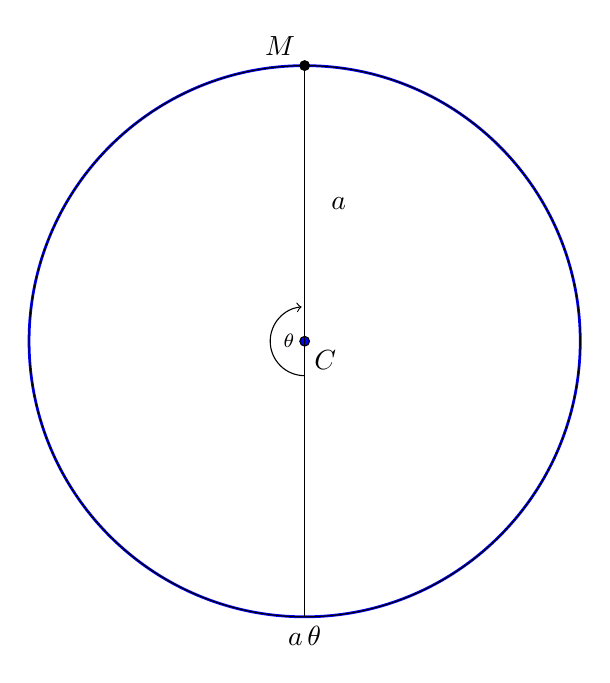
\begin{tikzpicture}[scale=3.5]
	\coordinate (O) at (0,0);
	\coordinate (A) at (0,2.5);
	\def\r{1} % radius
	\def\c{1.4} % center
	\coordinate (C) at (\c, \r);
	
	
	%	\draw[-latex] (O) -- (A) node[anchor=south] {$y$};
	%	\draw[-latex] (O) -- (1.1*pi,0) node[anchor=west] {$x$};
	%	\draw[red,domain=0:1*pi,samples=50, line width=1] 
	%	plot ({\x - sin(\x r)},{1 - cos(\x r)});
	\draw[blue, line width=1] (C) circle (\r);
	\draw[] (C) circle (\r);
	
	% coordinate x 
	\def\x{1.4} % coordinate x
	\def\y{2} % coordinate y
	\def\xa{0.3} % coordinate x for arc left
	\def\ya{1.2} % coordinate y for arc left
	\coordinate (X) at (\x, 0 );
	\coordinate (Y) at (0, \y );
	\coordinate (XY) at (\x, \y );
	\coordinate (XY) at (\x, \y );
	\coordinate (CY) at (\c, \y);
	
	%	\node[anchor=north] at (X) {$x$} ;
	
	% draw center of circle
	\draw[fill=blue] (C) circle (0.5pt);
	
	% draw radius of the circle
	\draw[] (C) -- node[anchor=west] {\; $a$} (XY);
	\node[anchor=north west] at (C) {$C$};
	
	% bottom of circle, radius to the bottom
	\coordinate (B) at (\c, 0);
	\draw[] (C) -- (B) node[anchor=north] {$a \, \theta$};
	
	%	% arc theta
	%	% start arc
	\coordinate (S) at (\c, 0.875);
	\draw[->] (S) arc (-90:-265:0.125);
	\node[xshift=-2mm, yshift=0mm] at (C) {\scriptsize $\theta$};
	
	% XY dot
	\draw[fill=black] (XY) circle (0.5pt);
	\node[anchor=south east] at (XY) {$M$};
	\end{tikzpicture}
	\caption{Case 7: $\theta = \pi$}
\end{figure}
In this case, we can see that
\begin{align}
\begin{cases}
\sin(\theta) &= 0\\
\cos(\theta) &= -1
\end{cases}
\end{align}
Therefore, the coordinate of $M$ is
\begin{align}
\begin{cases}
x(\theta) &= a \pi = a\left(\theta - \sin(\theta)\right)\\
y(\theta) &= 2 a = a\left(1 - \cos(\theta)\right)
\end{cases}
\end{align}

\newpage
\textbf{Case 8:} $\theta = \frac{3\pi}{2}$
\begin{figure}[H]
	\centering
	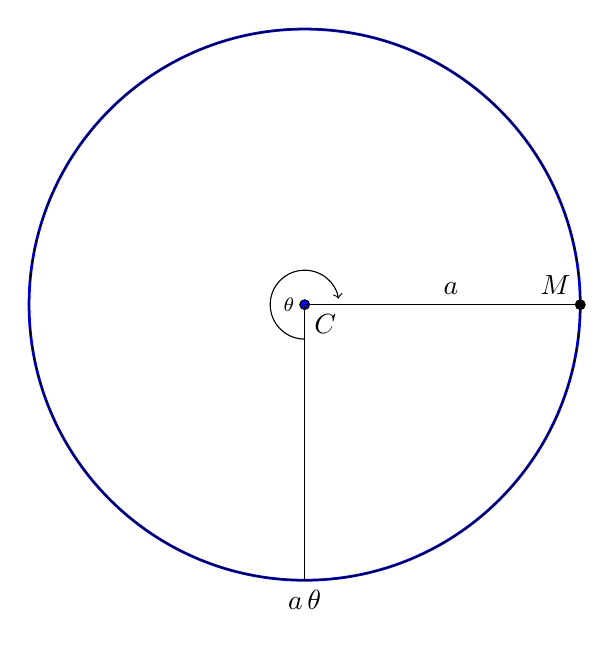
\begin{tikzpicture}[scale=3.5]
	\coordinate (O) at (0,0);
	\coordinate (A) at (0,2.5);
	\def\r{1} % radius
	\def\c{1.4} % center
	\coordinate (C) at (\c, \r);
	
	
	%	\draw[-latex] (O) -- (A) node[anchor=south] {$y$};
	%	\draw[-latex] (O) -- (1.1*pi,0) node[anchor=west] {$x$};
	%	\draw[red,domain=0:1*pi,samples=50, line width=1] 
	%	plot ({\x - sin(\x r)},{1 - cos(\x r)});
	\draw[blue, line width=1] (C) circle (\r);
	\draw[] (C) circle (\r);
	
	% coordinate x 
	\def\x{2.4} % coordinate x
	\def\y{1} % coordinate y
	\def\xa{0.3} % coordinate x for arc left
	\def\ya{1.2} % coordinate y for arc left
	\coordinate (X) at (\x, 0 );
	\coordinate (Y) at (0, \y );
	\coordinate (XY) at (\x, \y );
	\coordinate (XY) at (\x, \y );
	\coordinate (CY) at (\c, \y);
	
	%	\node[anchor=north] at (X) {$x$} ;
	
	% draw center of circle
	\draw[fill=blue] (C) circle (0.5pt);
	
	% draw radius of the circle
	\draw[] (C) -- node[anchor=south] {\; $a$} (XY);
	\node[anchor=north west] at (C) {$C$};
	
	% bottom of circle, radius to the bottom
	\coordinate (B) at (\c, 0);
	\draw[] (C) -- (B) node[anchor=north] {$a \, \theta$};
	
	% arc theta
	\coordinate (S) at (\c, 0.875);
	\draw[->] (S) arc (-90:-350:0.125);
	\node[xshift=-2mm, yshift=0mm] at (C) {\scriptsize $\theta$};
	
	% XY dot
	\draw[fill=black] (XY) circle (0.5pt);
	\node[anchor=south east] at (XY) {$M$};
	\end{tikzpicture}
	\caption{Case 8: $\theta = \frac{3\pi}{2}$}
\end{figure}
In this case, we can see that
\begin{align}
\begin{cases}
\sin(\theta) &= -1\\
\cos(\theta) &= 0
\end{cases}
\end{align}
Therefore, the coordinate of $M$ is
\begin{align}
\begin{cases}
x(\theta) &= a\pi + a = a\left(\theta - \sin(\theta)\right)\\
y(\theta) &= a = a\left(1 - \cos(\theta)\right)
\end{cases}
\end{align}

\newpage
\textbf{Case 9:} $\theta = 2\pi$
\begin{figure}[H]
	\centering
	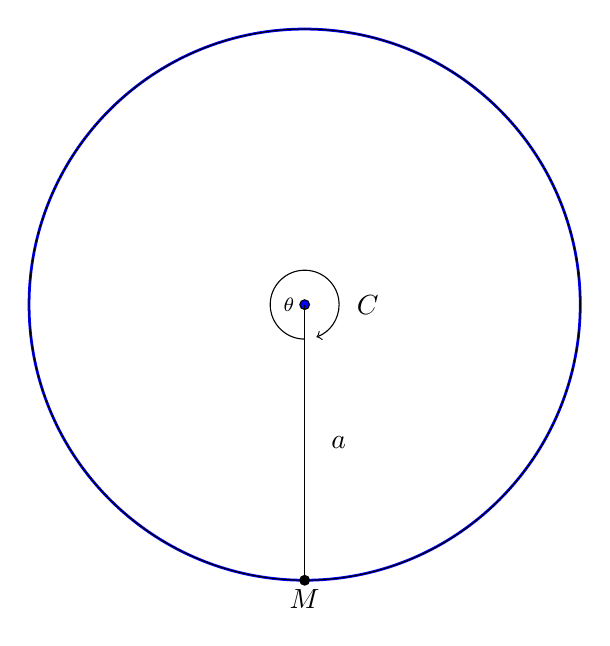
\begin{tikzpicture}[scale=3.5]
	\coordinate (O) at (0,0);
	\coordinate (A) at (0,2.5);
	\def\r{1} % radius
	\def\c{1.4} % center
	\coordinate (C) at (\c, \r);
	
	
	%	\draw[-latex] (O) -- (A) node[anchor=south] {$y$};
	%	\draw[-latex] (O) -- (1.1*pi,0) node[anchor=west] {$x$};
	%	\draw[red,domain=0:1*pi,samples=50, line width=1] 
	%	plot ({\x - sin(\x r)},{1 - cos(\x r)});
	\draw[blue, line width=1] (C) circle (\r);
	\draw[] (C) circle (\r);
	
	% coordinate x 
	\def\x{1.4} % coordinate x
	\def\y{0} % coordinate y
	\def\xa{0.3} % coordinate x for arc left
	\def\ya{1.2} % coordinate y for arc left
	\coordinate (X) at (\x, 0 );
	\coordinate (Y) at (0, \y );
	\coordinate (XY) at (\x, \y );
	\coordinate (XY) at (\x, \y );
	\coordinate (CY) at (\c, \y);
	
	%	\node[anchor=north] at (X) {$x$} ;
	
	% draw center of circle
	\draw[fill=blue] (C) circle (0.5pt);
	
	% draw radius of the circle
	\draw[] (C) -- node[anchor=west] {\; $a$} (XY);
	\node[xshift=8mm, yshift=0mm] at (C) {$C$};
	
	% arc theta
	\coordinate (S) at (\c, 0.875);
	\draw[->] (S) arc (-90:-430:0.125);
	\node[xshift=-2mm, yshift=0mm] at (C) {\scriptsize $\theta$};
	
	% XY dot
	\draw[fill=black] (XY) circle (0.5pt);
	\node[anchor=north] at (XY) {$M$};
	\end{tikzpicture}
	\caption{Case 9: $\theta = 2\pi$}
\end{figure}
In this case, we can see that
\begin{align}
\begin{cases}
\sin(\theta) &= 0\\
\cos(\theta) &= 1
\end{cases}
\end{align}
Therefore, the coordinate of $M$ is
\begin{align}
\begin{cases}
x(\theta) &= a 2 \pi = a\left(\theta - \sin(\theta)\right)\\
y(\theta) &= 0 = a\left(1 - \cos(\theta)\right)
\end{cases}
\end{align}

\newpage
Now, we have a parameterization of the cycloid
\begin{align}
	r(\theta) &= \left(x(\theta), y(\theta)\right) \\
	&= \left( a\left(\theta - \sin(\theta)\right), a\left(1 - \cos(\theta)\right)\right)
\end{align}
We can proceed to compute the curvature of the cycloid with $0 < \theta < 2\pi$. We have
\begin{align}
\begin{cases}
x' = \dfrac{d x}{d \theta} &= a - a\cos(\theta)\\
x'' = \dfrac{d^2 x}{d \theta^2} &= a\sin(\theta)
\end{cases}
\end{align}
and
\begin{align}
\begin{cases}
y' = \dfrac{d y}{d \theta} &= a\sin(\theta)\\
y'' = \dfrac{d^2 y}{d \theta^2} &= a\cos(\theta)
\end{cases}
\end{align}
The curvature of the cycloid can be computed as
\begin{align}
	\kappa &= \frac{x'y'' - y'x''}{\left(x'^2 + y'^2\right)^{\frac{3}{2}}} \\
	&= \frac{(a - a\cos(\theta))a\cos(\theta) - a\sin(\theta)a\sin(\theta)}{\left((a - a\cos(\theta))^2 + (a\sin(\theta))^2\right)^{\frac{3}{2}}} \\
	&= \frac{a^2\cos(\theta) - a^2\cos^2(\theta) - a^2\sin^2(\theta)}{\left(a^2 -2a^2\cos(\theta) + a^2\cos^2(\theta) + a^2\sin^2(\theta)\right)^{\frac{3}{2}}} \\
	&= \frac{a^2\cos(\theta) - a^2}{\left(a^2 -2a^2\cos(\theta) + a^2\right)^{\frac{3}{2}}} \\
	&= \frac{a^2(\cos(\theta) - 1)}{a^3\left(2-2\cos(\theta)\right)^{\frac{3}{2}}} \\
	&= -\frac{1-\cos(\theta)}{2^{\frac{3}{2}}a\left(1-\cos(\theta)\right)^{\frac{3}{2}}} \\
	&= -\frac{1}{2^{\frac{3}{2}}a\left(1-\cos(\theta)\right)^{\frac{1}{2}}} \\
	&= -\frac{1}{4a\frac{1}{\sqrt{2}}\left(1-\cos(\theta)\right)^{\frac{1}{2}}} \\
	&= -\frac{\sqrt{2}}{4a\left(1-\cos(\theta)\right)^{\frac{1}{2}}}
\end{align}

\newpage
\printindex
\newpage
\begin{thebibliography}{999}
\bibitem {1} \url{https://tex.stackexchange.com/questions/196957/how-can-i-draw-this-cycloid-diagram-with-tikz} 
\end{thebibliography}
\end{document}